\documentclass[tikz,margin=2mm]{standalone}
\usetikzlibrary{trees,arrows}
\begin{document}
\tikzstyle{level 1}=[level distance=30mm, sibling distance=30mm]
\tikzstyle{level 2}=[level distance=30mm, sibling distance=12mm]
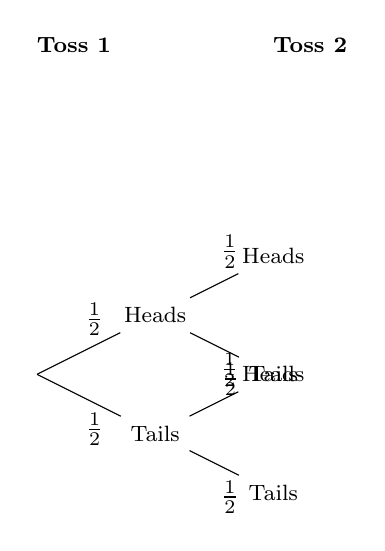
\begin{tikzpicture}[grow=right,-,>=angle 60]
%\begin{scope}[yshift=0]
  \coordinate
    child {node {\footnotesize Tails}%branch 1
      child {node {\footnotesize Tails}
      %probability dotted line insert below
        edge from parent
        node[pos = 0.5, below, yshift = -0.1cm, xshift = 0.2cm] (A1) {$\frac{1}{2}$}
      }
      child {node{\footnotesize Heads}
        edge from parent
        node[pos = 0.5, above, xshift = 0.2cm, yshift = 0.1cm] (A2) {$\frac{1}{2}$}
      }
      % child {node{$A_{2,2}$}
      % }
      %probability dotted line insert below
      edge from parent
        node[pos = 0.5, below, yshift = -0.1cm, xshift = 0.2cm] (A) {$\frac{1}{2}$}
        %condition Label
        node[pos = 1, above left, yshift = 4.5cm] (L) {\footnotesize \textbf{Toss 1}}
        node[pos = 1, above left, yshift = 4.5cm, xshift = 3cm] (L) {\footnotesize \textbf{Toss 2}}
    }
    child {node {\footnotesize Heads}
      child {node{\footnotesize Tails}
        edge from parent
        node[pos = 0.5, below, yshift = -0.1cm, xshift = 0.2cm] (B1) {$\frac{1}{2}$}
      }
      child {node{\footnotesize Heads}
        edge from parent
        node[pos = 0.5, above, xshift = 0.2cm, yshift = 0.1cm] (B2) {$\frac{1}{2}$}
      }
      % child {node{$A_{2,2}$}
      % }
      edge from parent
        node[pos = 0.5, above, xshift = 0.2cm, yshift = 0.1cm] (B) {$\frac{1}{2}$}
    }
    ;

\end{tikzpicture}

%Q2
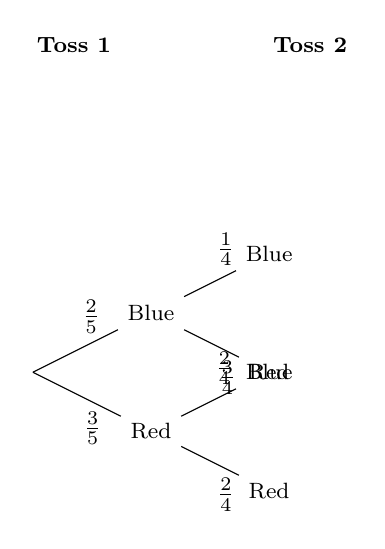
\begin{tikzpicture}[grow=right,-,>=angle 60]
%\begin{scope}[yshift=0]
  \coordinate
    child {node {\footnotesize Red}%branch 1
      child {node {\footnotesize Red}
      %probability dotted line insert below
        edge from parent
        node[pos = 0.5, below, yshift = -0.1cm, xshift = 0.2cm] (A1) {$\frac{2}{4}$}
      }
      child {node{\footnotesize Blue}
        edge from parent
        node[pos = 0.5, above, xshift = 0.2cm, yshift = 0.1cm] (A2) {$\frac{2}{4}$}
      }
      % child {node{$A_{2,2}$}
      % }
      %probability dotted line insert below
      edge from parent
        node[pos = 0.5, below, yshift = -0.1cm, xshift = 0.2cm] (A) {$\frac{3}{5}$}
        %condition Label
        node[pos = 1, above left, yshift = 4.5cm] (L) {\footnotesize \textbf{Toss 1}}
        node[pos = 1, above left, yshift = 4.5cm, xshift = 3cm] (L) {\footnotesize \textbf{Toss 2}}
    }
    child {node {\footnotesize Blue}
      child {node{\footnotesize Red}
        edge from parent
        node[pos = 0.5, below, yshift = -0.1cm, xshift = 0.2cm] (B1) {$\frac{3}{4}$}
      }
      child {node{\footnotesize Blue}
        edge from parent
        node[pos = 0.5, above, xshift = 0.2cm, yshift = 0.1cm] (B2) {$\frac{1}{4}$}
      }
      % child {node{$A_{2,2}$}
      % }
      edge from parent
        node[pos = 0.5, above, xshift = 0.2cm, yshift = 0.1cm] (B) {$\frac{2}{5}$}
    }
    %uncomment below to add another branch at level 1
    % child {node {$A_{2,1}$}
    %   child {node{$A_{3,2}$}
        
    %   }
    %   child {node{$A_{3,1}$}
    %   }
    % child {node{$A_{2,2}$}
    %   }
    %   edge from parent
    %     node[pos = 0.6, above, yshift = 0.2cm, xshift = 0.2cm] (C) {}
    % }
    ;
    

\end{tikzpicture}

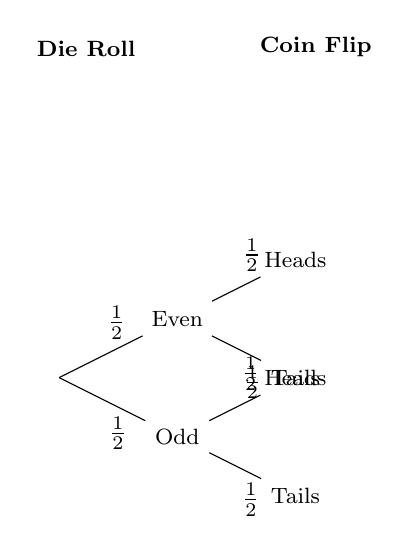
\begin{tikzpicture}[grow=right,-,>=angle 60]
%\begin{scope}[yshift=0]
  \coordinate
    child {node {\footnotesize Odd}%branch 1
      child {node {\footnotesize Tails}
      %probability dotted line insert below
        edge from parent
        node[pos = 0.5, below, yshift = -0.1cm, xshift = 0.2cm] (A1) {$\frac{1}{2}$}
      }
      child {node{\footnotesize Heads}
        edge from parent
        node[pos = 0.5, above, xshift = 0.2cm, yshift = 0.1cm] (A2) {$\frac{1}{2}$}
      }
      % child {node{$A_{2,2}$}
      % }
      %probability dotted line insert below
      edge from parent
        node[pos = 0.5, below, yshift = -0.1cm, xshift = 0.2cm] (A) {$\frac{1}{2}$}
        %condition Label
        node[pos = 1, above left, yshift = 4.5cm] (L) {\footnotesize \textbf{Die Roll}}
        node[pos = 1, above left, yshift = 4.5cm, xshift = 3cm] (L) {\footnotesize \textbf{Coin Flip}}
    }
    child {node {\footnotesize Even}
      child {node{\footnotesize Tails}
        edge from parent
        node[pos = 0.5, below, yshift = -0.1cm, xshift = 0.2cm] (B1) {$\frac{1}{2}$}
      }
      child {node{\footnotesize Heads}
        edge from parent
        node[pos = 0.5, above, xshift = 0.2cm, yshift = 0.1cm] (B2) {$\frac{1}{2}$}
      }
      % child {node{$A_{2,2}$}
      % }
      edge from parent
        node[pos = 0.5, above, xshift = 0.2cm, yshift = 0.1cm] (B) {$\frac{1}{2}$}
    }
    ;


\end{tikzpicture}

%Q4
\begin{tikzpicture}[grow=right,-,>=angle 60]
%\begin{scope}[yshift=0]
  \coordinate
    child {node {\footnotesize Boy}%branch 1
      child {node {\footnotesize Boy}
      %probability dotted line insert below
        edge from parent
        node[pos = 0.5, below, yshift = -0.1cm, xshift = 0.2cm] (A1) {$\frac{1}{2}$}
      }
      child {node{\footnotesize Girl}
        edge from parent
        node[pos = 0.5, above, xshift = 0.2cm, yshift = 0.1cm] (A2) {$\frac{1}{2}$}
      }
      % child {node{$A_{2,2}$}
      % }
      %probability dotted line insert below
      edge from parent
        node[pos = 0.5, below, yshift = -0.1cm, xshift = 0.2cm] (A) {$\frac{1}{2}$}
        %condition Label
        node[pos = 1, above left, yshift = 4.5cm] (L) {\footnotesize \textbf{$1^{st}$ Child}}
        node[pos = 1, above left, yshift = 4.5cm, xshift = 3cm] (L) {\footnotesize \textbf{$2^{nd}$ Child}}
    }
    child {node {\footnotesize Girl}
      child {node{\footnotesize Boy}
        edge from parent
        node[pos = 0.5, below, yshift = -0.1cm, xshift = 0.2cm] (B1) {$\frac{1}{2}$}
      }
      child {node{\footnotesize Girl}
        edge from parent
        node[pos = 0.5, above, xshift = 0.2cm, yshift = 0.1cm] (B2) {$\frac{1}{2}$}
      }
      % child {node{$A_{2,2}$}
      % }
      edge from parent
        node[pos = 0.5, above, xshift = 0.2cm, yshift = 0.1cm] (B) {$\frac{1}{2}$}
    }
    ;
\end{tikzpicture}


%Q5
\begin{tikzpicture}[grow=right,-,>=angle 60]
%\begin{scope}[yshift=0]
  \coordinate
    child {node {\footnotesize A}%branch 1
      child {node {\footnotesize A}
      %probability dotted line insert below
        edge from parent
        node[pos = 0.5, below, yshift = -0.1cm, xshift = 0.2cm] (A1) {$\frac{1}{4}$}
      }
      child {node{\footnotesize B}
        edge from parent
        node[pos = 0.5, above, xshift = 0.2cm, yshift = 0.1cm] (A2) {$\frac{1}{4}$}
      }
      % child {node{$A_{2,2}$}
      % }
      %probability dotted line insert below
      edge from parent
        node[pos = 0.5, below, yshift = -0.1cm, xshift = 0.2cm] (A) {$\frac{1}{4}$}
        %condition Label
        node[pos = 1, above left, yshift = 4.5cm] (L) {\footnotesize \textbf{$1^{st}$ Spin}}
        node[pos = 1, above left, yshift = 4.5cm, xshift = 3cm] (L) {\footnotesize \textbf{$2^{nd}$ Spin}}
    }
    child {node {\footnotesize B}
      child {node{\footnotesize A}
        edge from parent
        node[pos = 0.5, below, yshift = -0.1cm, xshift = 0.2cm] (B1) {$\frac{1}{4}$}
      }
      child {node{\footnotesize B}
        edge from parent
        node[pos = 0.5, above, xshift = 0.2cm, yshift = 0.1cm] (B2) {$\frac{1}{4}$}
      }
      % child {node{$A_{2,2}$}
      % }
      edge from parent
        node[pos = 0.5, above, xshift = 0.2cm, yshift = 0.1cm] (B) {$\frac{1}{4}$}
    }
    ;

\end{tikzpicture}

%Q6
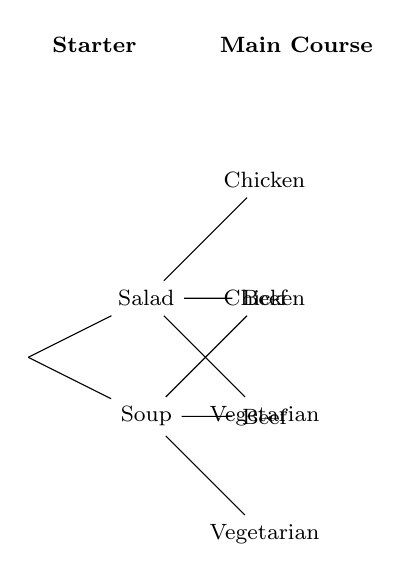
\begin{tikzpicture}[grow=right,-,>=angle 60]
%\begin{scope}[yshift=0]
  \coordinate
    child {node {\footnotesize Soup}%branch 1
      child {node {\footnotesize Vegetarian}
      }
      child {node{\footnotesize Beef}
      }
      child {node{\footnotesize Chicken}
      }
        %condition Label
        node[pos = 1, above left, yshift = 4.5cm] (L) {\footnotesize \textbf{Starter}}
        node[pos = 1, above left, yshift = 4.5cm, xshift = 3cm] (L) {\footnotesize \textbf{Main Course}}
    }
    child {node {\footnotesize Salad}
      child {node {\footnotesize Vegetarian}
      }
      child {node{\footnotesize Beef}
      }
      child {node{\footnotesize Chicken}
      }
    }
    ;
\end{tikzpicture}

%Q7
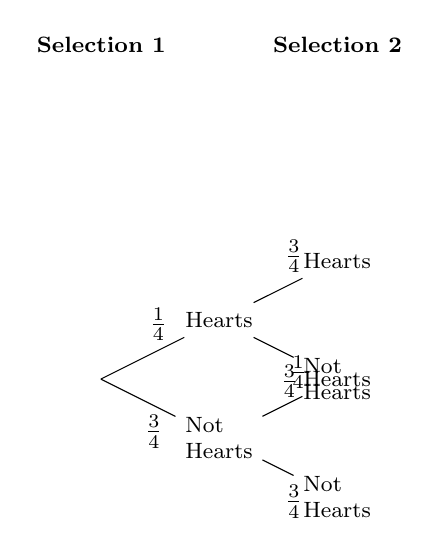
\begin{tikzpicture}[grow=right,-,>=angle 60]
%\begin{scope}[yshift=0]
  \coordinate
    child {node[align = left, font = \footnotesize ] {Not \\ Hearts}%branch 1
      child {node[align = left, font = \footnotesize ] {Not \\ Hearts}
      %probability dotted line insert below
        edge from parent
        node[pos = 0.5, below, yshift = -0.1cm, xshift = 0.2cm] (A1) {$\frac{3}{4}$}
      }
      child {node{\footnotesize Hearts}
        edge from parent
        node[pos = 0.5, above, xshift = 0.2cm, yshift = 0.1cm] (A2) {$\frac{1}{4}$}
      }
      % child {node{$A_{2,2}$}
      % }
      %probability dotted line insert below
      edge from parent
        node[pos = 0.5, below, yshift = -0.1cm, xshift = 0.2cm] (A) {$\frac{3}{4}$}
        %condition Label
        node[pos = 1, above left, yshift = 4.5cm] (L) {\footnotesize \textbf{Selection 1}}
        node[pos = 1, above left, yshift = 4.5cm, xshift = 3cm] (L) {\footnotesize \textbf{Selection 2}}
    }
    child {node {\footnotesize Hearts}
      child {node[align = left, font = \footnotesize ]{ Not \\ Hearts}
        edge from parent
        node[pos = 0.5, below, yshift = -0.1cm, xshift = 0.2cm] (B1) {$\frac{3}{4}$}
      }
      child {node{\footnotesize Hearts}
        edge from parent
        node[pos = 0.5, above, xshift = 0.2cm, yshift = 0.1cm] (B2) {$\frac{3}{4}$}
      }
      % child {node{$A_{2,2}$}
      % }
      edge from parent
        node[pos = 0.5, above, xshift = 0.2cm, yshift = 0.1cm] (B) {$\frac{1}{4}$}
    }
    ;
\end{tikzpicture}

%Q8
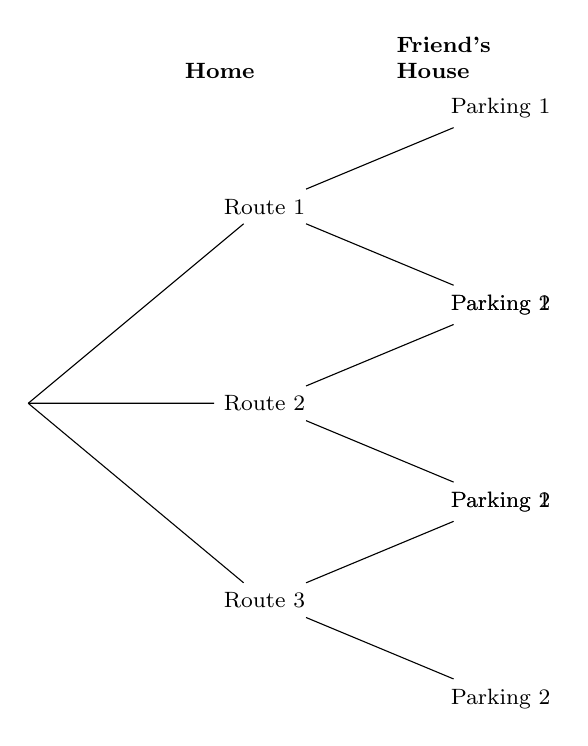
\begin{tikzpicture}[grow=right,-,>=angle 60]
\begin{scope}[yshift=0]
    \tikzstyle{level 1}=[level distance=30mm, sibling distance=25mm]
  \coordinate
    child {node {\footnotesize Route 3}%branch 1
      child {node[font = \footnotesize]{Parking 2}
      }
      child {node[font = \footnotesize]{Parking 1}
      }
      % child {node{$A_{2,2}$}
      % }
      %probability dotted line insert below
    }
    child {node[font = \footnotesize] { Route 2}
      child {node[font = \footnotesize]{Parking 2}
      }
      child {node[font = \footnotesize]{Parking 1}
      }
      % child {node{$A_{2,2}$}
      % }
    }
    %uncomment below to add another branch at level 1
    child {node[font = \footnotesize] {Route 1}
      child {node[font = \footnotesize]{Parking 2}
      }
      child {node[font = \footnotesize]{Parking 1}
      }
      %condition Label [ALWAYS ADD AFTER LAST CHILD NODE!]
        node[font = \footnotesize , pos = 1, above left, yshift = 1.5cm] (L) { \textbf{Home}}
        node[font = \footnotesize , align = left, pos = 1, above left, yshift = 1.5cm, xshift = 3cm] (L) {\textbf{Friend's} \\ \textbf{House}}
    % child {node{$A_{2,2}$}
    %   }
    }
    ;
\end{scope}
\end{tikzpicture}

%Q9
\begin{tikzpicture}[grow=right,-,>=angle 60]
%\begin{scope}[yshift=0]
  \coordinate
    child {node {\footnotesize No}%branch 1
      child {node {\footnotesize No}
      %probability dotted line insert below
        edge from parent
        node[pos = 0.5, below, yshift = -0.1cm, xshift = 0.2cm] (A1) {$\frac{1}{2}$}
      }
      child {node{\footnotesize Yes}
        edge from parent
        node[pos = 0.5, above, xshift = 0.2cm, yshift = 0.1cm] (A2) {$\frac{1}{2}$}
      }
      % child {node{$A_{2,2}$}
      % }
      %probability dotted line insert below
      edge from parent
        node[pos = 0.5, below, yshift = -0.1cm, xshift = 0.2cm] (A) {$\frac{1}{2}$}
        %condition Label
        node[pos = 1, above left, yshift = 4.5cm] (L) {\footnotesize \textbf{Round 1}}
        node[pos = 1, above left, yshift = 4.5cm, xshift = 3cm] (L) {\footnotesize \textbf{Round 2}}
    }
    child {node {\footnotesize Yes}
      child {node{\footnotesize No}
        edge from parent
        node[pos = 0.5, below, yshift = -0.1cm, xshift = 0.2cm] (B1) {$\frac{1}{2}$}
      }
      child {node{\footnotesize Yes}
        edge from parent
        node[pos = 0.5, above, xshift = 0.2cm, yshift = 0.1cm] (B2) {$\frac{1}{2}$}
      }
      % child {node{$A_{2,2}$}
      % }
      edge from parent
        node[pos = 0.5, above, xshift = 0.2cm, yshift = 0.1cm] (B) {$\frac{1}{2}$}
    }
    ;

\end{tikzpicture}

%Q10
\begin{tikzpicture}[grow=right,-,>=angle 60]
%\begin{scope}[yshift=0]
  \coordinate
    child {node {\footnotesize No}%branch 1
      child {node {\footnotesize No}
      %probability dotted line insert below
        edge from parent
        node[pos = 0.5, below, yshift = -0.1cm, xshift = 0.2cm] (A1) {$\frac{1}{2}$}
      }
      child {node{\footnotesize Yes}
        edge from parent
        node[pos = 0.5, above, xshift = 0.2cm, yshift = 0.1cm] (A2) {$\frac{1}{2}$}
      }
      % child {node{$A_{2,2}$}
      % }
      %probability dotted line insert below
      edge from parent
        node[pos = 0.5, below, yshift = -0.1cm, xshift = 0.2cm] (A) {$\frac{1}{2}$}
        %condition Label
        node[pos = 1, above left, yshift = 4.5cm] (L) {\footnotesize \textbf{Round 1}}
        node[pos = 1, above left, yshift = 4.5cm, xshift = 3cm] (L) {\footnotesize \textbf{Round 2}}
    }
    child {node {\footnotesize Yes}
      child {node{\footnotesize No}
        edge from parent
        node[pos = 0.5, below, yshift = -0.1cm, xshift = 0.2cm] (B1) {$\frac{1}{2}$}
      }
      child {node{\footnotesize Yes}
        edge from parent
        node[pos = 0.5, above, xshift = 0.2cm, yshift = 0.1cm] (B2) {$\frac{1}{2}$}
      }
      % child {node{$A_{2,2}$}
      % }
      edge from parent
        node[pos = 0.5, above, xshift = 0.2cm, yshift = 0.1cm] (B) {$\frac{1}{2}$}
    }
    ;

\end{tikzpicture}

%Q10
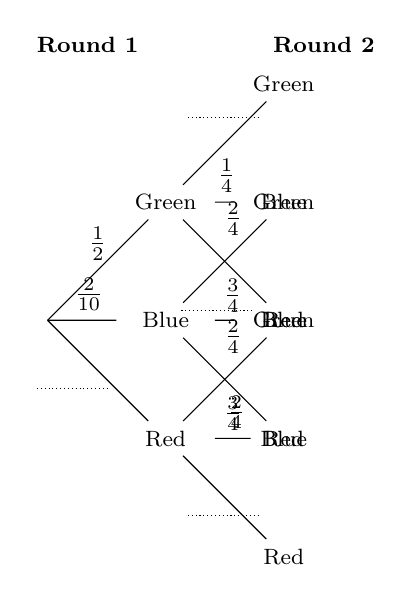
\begin{tikzpicture}[grow=right,-,>=angle 60]
  \coordinate
    child {node[font = \footnotesize, text width = 1cm, align = center] {Red}%branch 1
      child {node[font = \footnotesize] {Red}
      %probability dotted line insert below
      % [ADD LABEL AND UNCOMMENT THE DRAW LINE TO INSERT VALUE]
        edge from parent
        node[pos = 0.6, below] (A1) {}
      }
      child {node[font = \footnotesize]{Blue}
        edge from parent
        node[pos = 0.6, above] (A2) {$\frac{2}{4}$}
      }
      child {node[font = \footnotesize]{Green}
        edge from parent
        node[pos = 0.6, above,yshift = 0.1cm] (A3) {$\frac{2}{4}$}
      }
      %probability blank OR value inserted below [ADD LABEL AND UNCOMMENT THE DRAW LINE TO INSERT VALUE]
      edge from parent
        node[pos = 0.5, below, yshift = -0.1cm, xshift = -0.2cm] (A) {}
    }
    child {node[font = \footnotesize, text width = 1cm, align = center] {Blue}
      child {node[font = \footnotesize, text width = 1cm, align = center]{Red}
        edge from parent
        node[pos = 0.6, below] (B1) {$\frac{3}{4}$}
      }
      child {node[font = \footnotesize, text width = 1cm, align = center]{Blue}
        edge from parent
        node[pos = 0.6, above] (B2) {}
      }
      child {node[font = \footnotesize, text width = 1cm, align = center]{Green}
        edge from parent
        node[pos = 0.6, above, yshift = 0.1cm] (B3) {$\frac{2}{4}$}
      }
      edge from parent
        node[pos = 0.6, above] (B) {$\frac{2}{10}$}
    }
    %uncomment below to add another branch at level 1
    child {node[font = \footnotesize, text width = 1cm, align = center] {Green}
      child {node[font = \footnotesize, text width = 1cm, align = center]{Red}
        edge from parent
        node[pos = 0.6, below] (C1) {$\frac{3}{4}$}
      }
      child {node[font = \footnotesize, text width = 1cm, align = center]{Blue}
        edge from parent
        node[pos = 0.6, above] (C2) {$\frac{1}{4}$}
      }
      child {node[font = \footnotesize, text width = 1cm, align = center]{Green}
        edge from parent
        node[pos = 0.6, above, yshift = 0.1cm] (C3) {}
      }
        %probability dotted line insert below
      edge from parent
        node[pos = 0.5, above] (C) {$\frac{1}{2}$}
        %condition Label
        node[pos = 1, above left, yshift = 2cm] (L) {\footnotesize \textbf{Round 1}}
        node[pos = 1, above left, yshift = 2cm, xshift = 3cm] (L) {\footnotesize \textbf{Round 2}} 
    };

     %Blank Spaces (dotted lines)

    \draw [densely dotted, shorten >= -0.45cm, shorten <=-0.45cm] (A)-- ++(0:-0.1);
    \draw [densely dotted, shorten >= -0.45cm, shorten <=-0.45cm] (A1)-- ++(0:-0.1);
    % \draw [densely dotted, shorten >= -0.45cm, shorten <=-0.45cm] (A2)-- ++(0:-0.1);
    % \draw [densely dotted, shorten >= -0.45cm, shorten <=-0.45cm] (A3)-- ++(0:-0.1);
    % \draw [densely dotted, shorten >= -0.45cm, shorten <=-0.45cm] (B)-- ++(0:-0.1);
    % \draw [densely dotted, shorten >= -0.45cm, shorten <=-0.45cm] (B1)-- ++(0:-0.1);
    \draw [densely dotted, shorten >= -0.45cm, shorten <=-0.45cm] (B2)-- ++(0:-0.1);
    % \draw [densely dotted, shorten >= -0.45cm, shorten <=-0.45cm] (B3)-- ++(0:-0.1);
    % \draw [densely dotted, shorten >= -0.45cm, shorten <=-0.45cm] (C)-- ++(0:-0.1);
    % \draw [densely dotted, shorten >= -0.45cm, shorten <=-0.45cm] (C1)-- ++(0:-0.1);
    % \draw [densely dotted, shorten >= -0.45cm, shorten <=-0.45cm] (C2)-- ++(0:-0.1);
    \draw [densely dotted, shorten >= -0.45cm, shorten <=-0.45cm] (C3)-- ++(0:-0.1);
\end{tikzpicture}

\end{document}